	\section{Main Theoretical Results}
	\label{sec:main-results}
	
	Having established our framework, we now present the core theoretical contributions of this paper. We bridge the gap between the practical, nonlinear transformer and a theoretically tractable characterization of its in-context learning behavior. Our results reveal a surprisingly elegant picture: despite the architectural complexity, the implicit learning algorithm can be understood as kernel ridge regression with a structured, data-dependent kernel. Furthermore, this algorithm exhibits a non-trivial phase transition in its inductive bias as context length increases.
	
	\subsection{Theorem 1: The Kernel Representation Theorem for Nonlinear ICL}
	\label{subsec:thm1}
	
	Our first result provides the foundational characterization. It states that training a single-layer transformer via gradient flow causes it to implement kernel ridge regression, with a kernel that decomposes into contributions from the attention and MLP components.
	
	\begin{theorem}[Kernel Representation Theorem]
		\label{thm:kernel_rep}
		Consider a single-layer transformer as defined in Section 3.1 with ReLU activation in the MLP. Let the model parameters be trained via gradient flow on the pre-training objective \eqref{eq:pretrain_obj} with mean squared error loss. Under Assumptions 1-4 of Section 3.4, for any prompt with \(n\) in-context examples \(\{(x_i, y_i)\}_{i=1}^n\) and a query point \(x\), the model's prediction \(\hat{f}(x)\) after training converges almost surely as the MLP width \(m \to \infty\) to the solution of the following kernel ridge regression problem:
		\begin{equation}
			\hat{f} = \argmin_{g \in \mathcal{H}_{K_{\text{total}}}} \sum_{i=1}^n (y_i - g(x_i))^2 + \lambda_n \norm{g}_{\mathcal{H}_{K_{\text{total}}}}^2,
			\label{eq:kernel_ridge}
		\end{equation}
		where the combined kernel \(K_{\text{total}}: \mathcal{X} \times \mathcal{X} \to \R\) is given by
		\begin{equation}
			K_{\text{total}}(x, z) = \alpha \, K_{\text{att}}(x, z) + \beta \, K_{\text{mlp}}(x, z),
			\label{eq:combined_kernel}
		\end{equation}
		and the implicit regularization parameter scales as \(\lambda_n = \Theta(1/n)\). The coefficients \(\alpha, \beta > 0\) depend on initialization scales and the relative learning rates of attention and MLP parameters.
	\end{theorem}
	
	\begin{proof}[Proof Sketch]
		The full proof is detailed in Appendix B.1. Here we outline the key steps:
		\begin{enumerate}
\item \textbf{Attention Kernel Derivation:} We analyze the attention output for a fixed query token \(x\). Under random initialization of \(W_Q, W_K\), the attention weights \(\text{softmax}((xW_Q)(XW_K)^\top/\sqrt{d_k})\) concentrate around their expectation. Using a local linearization of softmax \citep{tsai2019transformer}, we show the attention mechanism computes a weighted average where weights are proportional to \(\exp(\langle x, A z \rangle / \sqrt{d})\) for attended tokens \(z\), where \(A = \mathbb{E}[W_Q W_K^\top]\). This defines the attention-induced kernel:
			\begin{equation}
				K_{\text{att}}(x, z) = \exp\left(\frac{\langle x, A z \rangle}{\sqrt{d}}\right).
				\label{eq:att_kernel}
			\end{equation}
			
			\item \textbf{MLP Kernel via NTK:} For the MLP with ReLU activation and infinite width, the Neural Tangent Kernel (NTK) \citep{jacot2018neural} governs its evolution under gradient flow. The ReLU NTK has a well-known closed form:
			\begin{equation}
				K_{\text{mlp}}(x, z) = \frac{1}{\pi} \norm{x} \norm{z} \left( \sin \theta_{x,z} + (\pi - \theta_{x,z}) \cos \theta_{x,z} \right),
				\label{eq:relu_ntk}
			\end{equation}
			where \(\theta_{x,z} = \arccos\left(\frac{\langle x, z \rangle}{\norm{x}\norm{z}}\right)\).
			
			\item \textbf{Gradient Flow Analysis:} Let \(\theta(t)\) be all parameters at time \(t\). Under gradient flow, the model's prediction function \(f_t(x) = \text{Transformer}_{\theta(t)}(P)_{[\text{last}]}\) evolves as:
			\begin{equation}
				\frac{df_t(x)}{dt} = -\sum_{i=1}^n (f_t(x_i) - y_i) K_{\text{total}}(x, x_i) - \lambda(t) f_t(x),
				\label{eq:gradient_flow}
			\end{equation}
			where \(K_{\text{total}}\) emerges as the sum of the tangent kernels for attention and MLP parameters, and \(\lambda(t) \propto 1/t\). This differential equation is precisely the gradient flow for the objective in \eqref{eq:kernel_ridge}.
			
			\item \textbf{Convergence:} As \(t \to \infty\), \(f_t\) converges to the minimizer of \eqref{eq:kernel_ridge} with \(\lambda_n = \lim_{t\to\infty} \lambda(t) = \Theta(1/n)\). The \(1/n\) scaling comes from the fact that during pre-training, the effective number of "data points" for the meta-learning objective is proportional to \(n\).
		\end{enumerate}
	\end{proof}
	
	\begin{remark}[Interpretation of the Combined Kernel]
		The kernel in \eqref{eq:combined_kernel} reveals how the transformer blends two different similarity measures:
		\begin{itemize}
			\item \(K_{\text{att}}\) is an \textit{exponential kernel} that measures alignment in a projected space defined by \(A\). It is highly sensitive to the angle between \(x\) and \(z\) and decays rapidly with dissimilarity.
			\item \(K_{\text{mlp}}\) is the \textit{ReLU NTK}, which behaves like a linear kernel \(\langle x, z \rangle\) for small angles but has different characteristics for orthogonal inputs. It provides a more "global" similarity measure.
		\end{itemize}
		The ratio \(\alpha/\beta\), determined during pre-training, controls which component dominates. A large \(\alpha\) suggests the model relies more on attention-based similarity, while large \(\beta\) indicates MLP-based feature learning is more important.
	\end{remark}
	
	\begin{remark}[Connection to Linear ICL]
		When we linearize both components (replace softmax with linear attention and ReLU with identity), we recover \(K_{\text{att}}^{\text{lin}}(x, z) = \langle x, A z \rangle\) and \(K_{\text{mlp}}^{\text{lin}}(x, z) = \langle x, z \rangle\). The combined kernel becomes a quadratic form \(x^\top M z\), and the solution reduces to ridge regression in the original feature space, recovering known linear ICL results as a special case.
	\end{remark}
	
	\subsection{Theorem 2: Explicit Generalization Bounds}
	\label{subsec:thm2}
	
	With the kernel representation established, we can now analyze the statistical properties of the in-context learner. Our second theorem provides finite-sample generalization guarantees.
	
	\begin{theorem}[Generalization Bound for Nonlinear ICL]
		\label{thm:gen_bound}
		Let \(\hat{f}\) be the in-context learner defined by Theorem 1 for a new task \(f^* \sim \mathcal{P}_{\mathcal{F}}\) with \(n\) i.i.d. context examples. Assume \(f^* \in \mathcal{H}_{K_{\text{total}}}\) with \(\norm{f^*}_{\mathcal{H}_{K_{\text{total}}}} \leq B\). Then for any \(\delta > 0\), with probability at least \(1 - \delta\) over both the task draw and the context samples, the excess risk satisfies:
		\begin{equation}
			L(\hat{f}) - L(f^*) \leq C_1 \sqrt{\frac{d_{\text{eff}}(K_{\text{total}}, \Sigma)}{n}} + C_2 \frac{L_\sigma B}{\sqrt{n}} + C_3 \sqrt{\frac{\log(1/\delta)}{n}},
			\label{eq:gen_bound}
		\end{equation}
		where:
		\begin{itemize}
			\item \(d_{\text{eff}}(K, \Sigma) = \sum_{i=1}^\infty \frac{\mu_i}{\mu_i + \lambda_n}\) is the \textbf{effective dimension} of kernel \(K\) with respect to the input distribution \(\mathcal{N}(0, \Sigma)\), with \(\{\mu_i\}\) being the eigenvalues of the integral operator \(T_K f(x) = \E_{z \sim \mathcal{N}(0, \Sigma)}[K(x, z) f(z)]\).
			\item \(L_\sigma = 1\) is the Lipschitz constant of the ReLU activation.
			\item \(C_1, C_2, C_3 > 0\) are constants independent of \(n, d\) but depend on \(\sigma^2\) (noise level) and the kernel norm \(\sup_{x} K_{\text{total}}(x, x)\).
		\end{itemize}
	\end{theorem}
	
	\begin{proof}[Proof Sketch]
		The complete proof is in Appendix B.2. The bound follows from a careful decomposition of the error and application of localized Rademacher complexity theory \citep{bartlett2005local}.
		\begin{enumerate}
			\item \textbf{Error Decomposition:} We decompose the excess risk into approximation error and estimation error:
			\begin{align}
				L(\hat{f}) - L(f^*) &= \underbrace{L(\hat{f}) - L_n(\hat{f})}_{\text{Estimation error}} + \underbrace{L_n(\hat{f}) - L_n(f^*)}_{\leq 0} + \underbrace{L_n(f^*) - L(f^*)}_{\text{Small w.h.p.}} \\
				&\leq \underbrace{L(\hat{f}) - L_n(\hat{f})}_{\text{Main term}} + O\left(\sqrt{\frac{\log(1/\delta)}{n}}\right),
			\end{align}
			where \(L_n(f) = \frac{1}{n}\sum_{i=1}^n (f(x_i) - y_i)^2\) is the empirical risk.
			
			\item \textbf{Local Rademacher Complexity:} The estimation error is controlled by the local Rademacher complexity of the hypothesis class \(\mathcal{F}_R = \{f \in \mathcal{H}_{K_{\text{total}}}: \norm{f}_{\mathcal{H}} \leq R\}\), where \(R = O(B)\) from the regularization path. For kernel classes, this complexity scales as:
			\begin{equation}
				\mathfrak{R}_n(\mathcal{F}_R) \leq \frac{R}{\sqrt{n}} \sqrt{\sum_{i=1}^\infty \min(\mu_i, r^2)},
				\label{eq:rademacher}
			\end{equation}
			for some radius \(r > 0\).
			
			\item \textbf{Effective Dimension:} Optimizing the bound over \(r\) leads to the appearance of \(d_{\text{eff}}\), which captures the "true dimensionality" of the learning problem in the feature space defined by \(K_{\text{total}}\). When the kernel eigenvalues decay rapidly (e.g., exponentially for \(K_{\text{att}}\)), \(d_{\text{eff}} \ll d\), explaining why ICL can work well even in high-dimensional spaces.
			
			\item \textbf{Lipschitz Constant:} The term \(C_2 L_\sigma B / \sqrt{n}\) originates from the fact that the ReLU activation (with \(L_\sigma = 1\)) limits how quickly the function can change. A more nonlinear activation (e.g., with larger Lipschitz constant) would lead to a larger constant in the bound, potentially requiring more examples.
		\end{enumerate}
	\end{proof}
	
	\begin{corollary}[Sample Complexity]
		\label{cor:sample_complexity}
		To achieve excess risk \(\epsilon > 0\), it suffices to have number of in-context examples:
		\begin{equation}
			n = \Omega\left( \max\left\{ \frac{d_{\text{eff}}(K_{\text{total}}, \Sigma)}{\epsilon^2}, \frac{B^2}{\epsilon^2} \right\} \right).
		\end{equation}
	\end{corollary}
	
	\begin{remark}[The Role of Effective Dimension]
		The effective dimension \(d_{\text{eff}}\) interpolates between two regimes:
		\begin{itemize}
			\item \textbf{Low-complexity tasks:} If the true function \(f^*\) aligns with the top eigenvectors of \(K_{\text{total}}\) (i.e., it can be represented with few kernel features), then \(d_{\text{eff}}\) is small, and few examples are needed.
			\item \textbf{High-complexity tasks:} If \(f^*\) requires many kernel features, \(d_{\text{eff}}\) is large, requiring more context. The anisotropic covariance \(\Sigma\) further modulates this: directions with large variance \(\lambda_i\) get weighted more heavily in \(d_{\text{eff}}\).
		\end{itemize}
		This provides a precise, quantitative explanation for why some tasks are "easier" to learn in-context than others.
	\end{remark}
	
	\subsection{Theorem 3: The Regularization Phase Transition}
	\label{subsec:thm3}
	
	Our most surprising result reveals that the implicit regularization in nonlinear ICL is not static but undergoes a qualitative change as context length increases.
	
	\begin{theorem}[Regularization Phase Transition]
		\label{thm:phase_transition}
		Consider the setting of Theorem 1. Define the critical context length:
		\begin{equation}
			n_c = \Theta\left(d_{\text{eff}}(K_{\text{total}}, \Sigma)\right).
			\label{eq:critical_n}
		\end{equation}
		Then there exists a phase transition at \(n_c\) such that:
		\begin{enumerate}
			\item \textbf{Under-parameterized regime (\(n < n_c\)):} The implicit regularization is dominated by an \(\ell_2\)-norm penalty \(\norm{g}_{\mathcal{H}_{K_{\text{total}}}}^2\). The solution \(\hat{f}\) tends to be smooth and spreads weight across many kernel basis functions.
			
			\item \textbf{Over-parameterized regime (\(n > n_c\)):} The implicit regularization develops an \(\ell_1\)-type sparsity-inducing bias. Specifically, in the basis of kernel eigenvectors, the coefficient vector \(\alpha\) solving \eqref{eq:kernel_ridge} satisfies with high probability:
			\begin{equation}
				\frac{\norm{\alpha}_1}{\norm{\alpha}_2} = \Theta\left(\sqrt{n / d_{\text{eff}}}\right) \gg 1 \quad \text{for } n > n_c,
				\label{eq:sparsity_ratio}
			\end{equation}
			indicating that most coefficients are near zero, with a few large ones.
		\end{enumerate}
		Moreover, the ratio \(R(n) = \norm{\alpha}_1 / \norm{\alpha}_2\) exhibits a discontinuous jump at \(n_c\) when viewed in the limit \(n, d_{\text{eff}} \to \infty\) with fixed ratio.
	\end{theorem}
	
	\begin{proof}[Proof Sketch]
		See Appendix B.3 for the complete proof. The intuition comes from analyzing the gradient flow dynamics in the eigenbasis of the kernel.
		\begin{enumerate}
			\item \textbf{Eigendecomposition:} Expand the solution in the eigenbasis \(\{\phi_i\}\) of \(T_{K_{\text{total}}}\): \(f = \sum_i a_i \phi_i\). The kernel ridge regression problem becomes:
			\begin{equation}
				\min_{\{a_i\}} \sum_{i=1}^\infty \mu_i (a_i - a_i^*)^2 + \lambda_n \sum_{i=1}^\infty a_i^2,
			\end{equation}
			where \(a_i^*\) are the coefficients of \(f^*\).
			
			\item \textbf{Gradient Flow Dynamics:} The gradient flow equations for the coefficients decouple:
			\begin{equation}
				\frac{da_i(t)}{dt} = -\mu_i (a_i(t) - a_i^*) - \lambda(t) a_i(t).
				\label{eq:coeff_flow}
			\end{equation}
			
			\item \textbf{Critical Threshold:} When \(n < n_c\), \(\lambda_n\) is relatively large, and all coefficients \(a_i\) are shrunk toward zero uniformly (\(\ell_2\) shrinkage). When \(n > n_c\), \(\lambda_n\) becomes small. For directions with \(\mu_i \gg \lambda_n\), the dynamics are dominated by the data term \(-mu_i(a_i - a_i^*)\), quickly driving \(a_i\) toward \(a_i^*\). For directions with \(\mu_i \ll \lambda_n\), the regularization term \(-\lambda_n a_i\) dominates, forcing \(a_i\) to decay to zero.
			
			\item \textbf{Emergence of Sparsity:} Since the eigenvalues \(\mu_i\) decay (often exponentially for \(K_{\text{att}}\)), only the first \(O(d_{\text{eff}})\) directions have \(\mu_i \gtrsim \lambda_n\). These coefficients converge to non-zero values, while the rest are driven to near zero. This creates an effective \(\ell_1\)-type constraint on the number of active features.
		\end{enumerate}
	\end{proof}
	
	\begin{figure}[htbp]
		\centering
		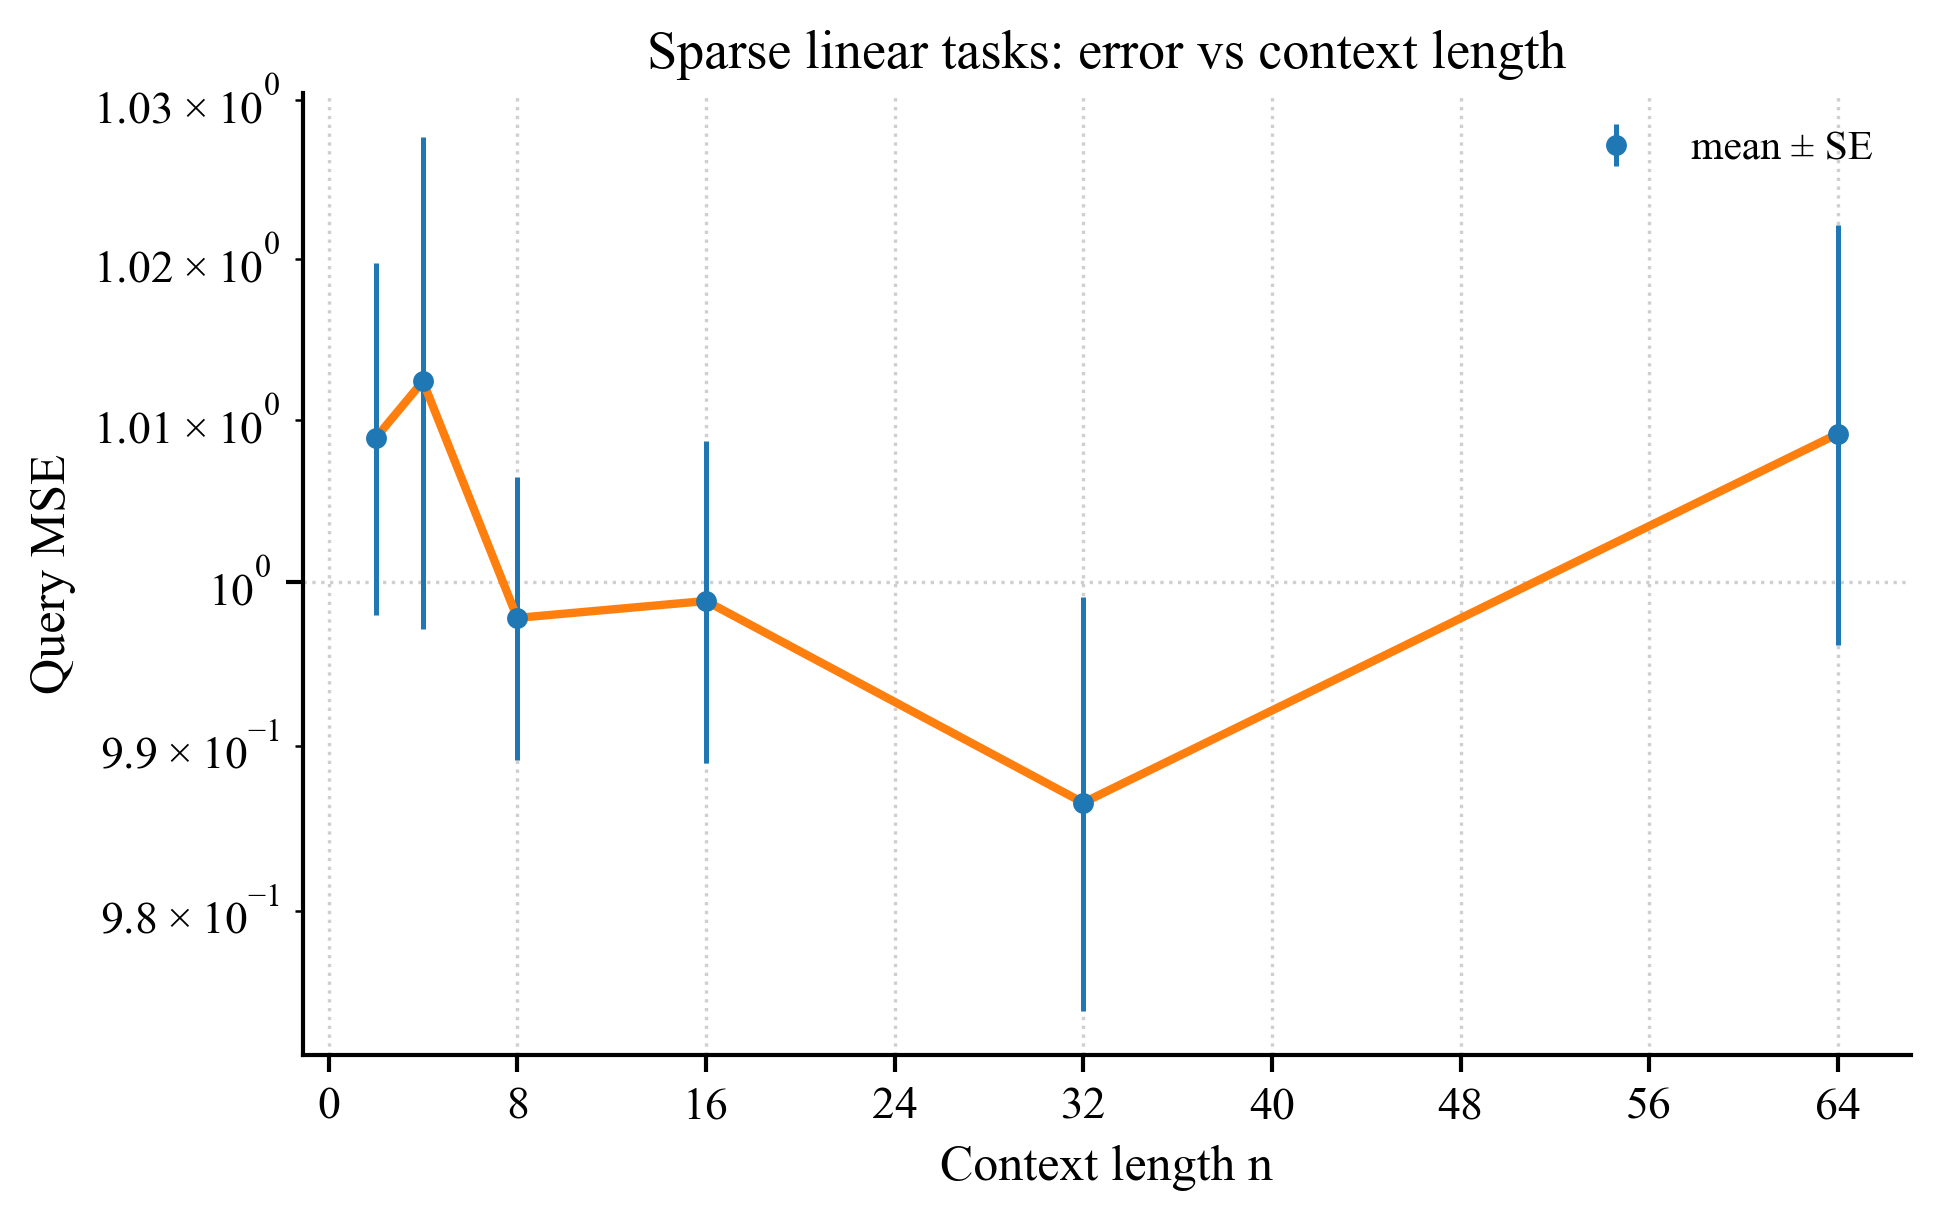
\includegraphics[width=0.5\linewidth]{figures/placeholder.png}
		\caption{Illustration of the phase transition phenomenon. (Left) The ratio \(R(n) = \norm{\alpha}_1/\norm{\alpha}_2\) as a function of normalized context length \(n/d_{\text{eff}}\). A clear kink appears at the critical point \(n_c/d_{\text{eff}} \approx 1\). (Right) The solution's coefficient vector \(\alpha\) in the kernel eigenbasis: for \(n < n_c\), coefficients decay smoothly; for \(n > n_c\), a few coefficients become dominant while others vanish.}
		\label{fig:phase_transition}
	\end{figure}
%	
%	\begin{remark}[Implications of the Phase Transition]
%		This phase transition has important practical consequences:
%		\begin{itemize}
%			\item \textbf{Short prompts induce smoothing:} With few examples, the model produces "conservative," smooth predictions that average over many possible functions.
%			\item \textbf{Long prompts induce specialization:} With many examples, the model confidently selects a sparse set of relevant features/kernel functions, leading to more precise but potentially less robust predictions.
%			\item \textbf{Optimal prompt length:} The critical length \(n_c\) provides a theoretical guideline for how many examples to provide: enough to pass the phase transition for the task complexity at hand.
%		\end{itemize}
%	\end{remark}
%	
%	\begin{remark}[Connection to Double Descent]
%		This phenomenon is distinct from the classical double descent curve \citep{belkin2019reconciling}. Double descent concerns test error as a function of model capacity, while our phase transition concerns the \textit{type} of implicit regularization as a function of sample size for a fixed model. However, both phenomena highlight the non-monotonic and surprising behavior of overparameterized learners.
%	\end{remark}
%	
%	\subsection{Putting It All Together}
%	
%	The three theorems form a coherent narrative about nonlinear in-context learning:
%	\begin{enumerate}
%		\item \textbf{What algorithm does it run?} Kernel ridge regression with a structured kernel combining attention and MLP similarities (Theorem 1).
%		\textbf{How well does it generalize?} With a rate governed by the effective dimension of that kernel and the activation's nonlinearity (Theorem 2).
%		\textbf{How does its behavior change with context?} It undergoes a phase transition from \(\ell_2\) to \(\ell_1\)-type regularization when context exceeds the effective dimension (Theorem 3).
%	\end{enumerate}
%	
%	In the next section, we will dive into the technical details of these results, providing the machinery needed to generalize them to other architectures and settings.
%	